% Appendix A

\chapter{Appendix C - Model Graph} % Main appendix title

\label{AppendixC} % For referencing this appendix elsewhere, use \ref{AppendixA}

\begin{table}[!ht]
    \centering
    \caption{Sample Network Architecture for Spectrogram}
    \begin{tabular}{|l|l|l|}
    \hline
        \textbf{Layer (Type)} & \textbf{Output Shape} & \textbf{Number of Parameters} \\ \hline
        input (InputLayer) & "(None, None, 193)" & 0 \\ \hline
        expand\_dim (Reshape) & "(None, None, 193, 1)" & 0 \\ \hline
        conv\_1 (Conv2D) & "(None, None, 97, 32)" & 14432 \\ \hline
        conv\_1\_bn (BatchNormalization) & "(None, None, 97, 32)" & 128 \\ \hline
        conv\_1\_relu (ReLU) & "(None, None, 97, 32)" & 0 \\ \hline
        conv\_2 (Conv2D) & "(None, None, 49, 32)  " & 236544 \\ \hline
        conv\_2\_bn (BatchNormalization) & "(None, None, 49, 32)  " & 128 \\ \hline
        conv\_2\_relu (ReLU) & "(None, None, 49, 32)  " & 0 \\ \hline
        reshape\_1 (Reshape) & "(None, None, 1568)" & 0 \\ \hline
        bidirectionalLSTM\_1 (Bidirectional) & "(None, None, 1024)" & 8523776 \\ \hline
        dropout (Dropout) & "(None, None, 1024)" & 0 \\ \hline
        bidirectionalLSTM\_2 (Bidirectional) & "(None, None, 1024)" & 6295552 \\ \hline
        dropout\_1 (Dropout) & "(None, None, 1024)" & 0 \\ \hline
        bidirectionalLSTM\_3 (Bidirectional) & "(None, None, 1024)" & 6295552 \\ \hline
        dropout\_2 (Dropout) & "(None, None, 1024)" & 0 \\ \hline
        bidirectionalLSTM\_4 (Bidirectional) & "(None, None, 1024)" & 6295552 \\ \hline
        dropout\_3 (Dropout) & "(None, None, 1024)" & 0 \\ \hline
        bidirectionalLSTM\_5 (Bidirectional) & "(None, None, 1024)" & 6295552 \\ \hline
        dense\_1 (Dense) & "(None, None, 1024)" & 1049600 \\ \hline
        dense\_1\_relu (ReLU) & "(None, None, 1024)" & 0 \\ \hline
        dropout\_4 (Dropout) & "(None, None, 1024)" & 0 \\ \hline
        dense (Dense) & "(None, None, 32) " & 32800 \\ \hline
        \textbf{Total parameters} & ~ & 35039616 \\ \hline
    \end{tabular}
    \label{model}
\end{table}

\begin{figure}[th]
    \centering
    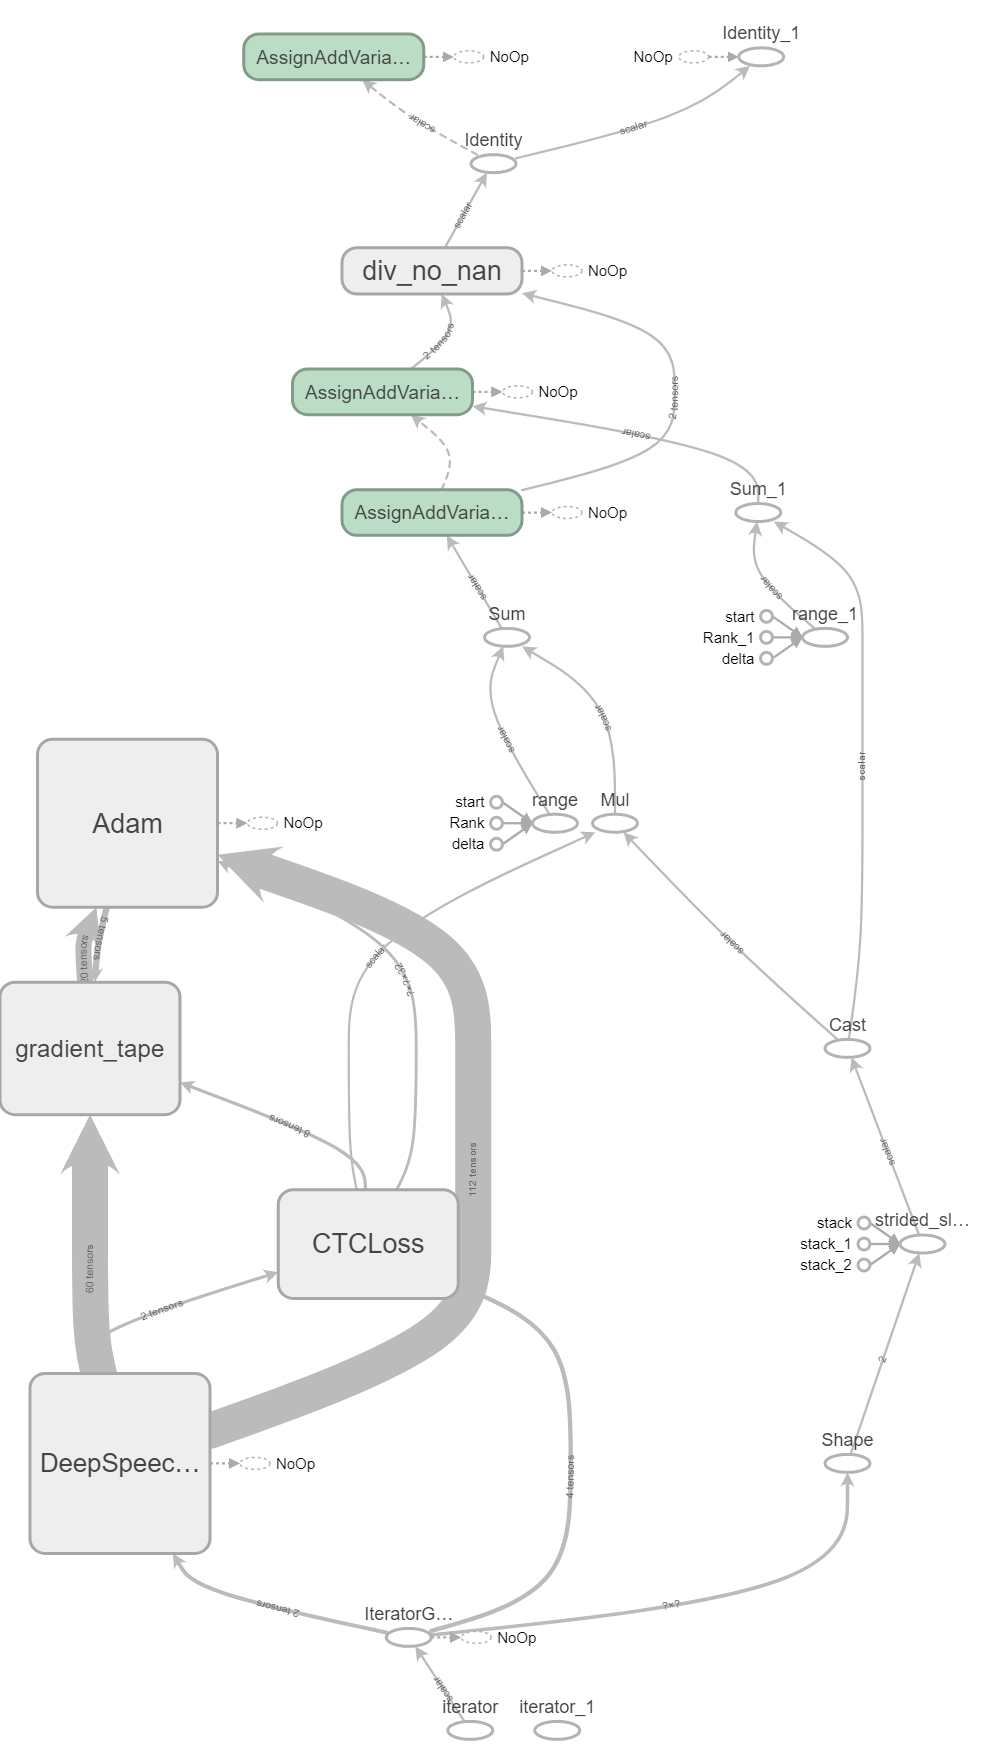
\includegraphics[width=0.7\textwidth]{Figures/model.png}
    \caption[TensorflowModelGraph]{A graph of the general Tensorflow model used in this investigation - deep speech is the name of the neural network outlined above}
    \label{fig:TensorflowModelGraph}
\end{figure}
